\documentclass{beamer}
\usetheme{Juelich}
\usepackage{helvet}
\usepackage{tikz,calc}
\usepackage{textpos} % package for the positioning
\usepackage{pgfplots}
\pgfplotsset{compat=newest}
\usetikzlibrary{arrows.meta}
\usetikzlibrary{math}
\usetikzlibrary{calc}
\usepackage{color}
\usepgfplotslibrary{groupplots} % Libraries to generate group plots
\usetikzlibrary{pgfplots.groupplots}


\title{SU(3) Interpolating operators}
\subtitle{@ SU(3) flavor degenerate point}
\author{Thomas Luu, IAS-4}
\date{\today}

\pgfdeclareimage[interpolate=true,width=4cm]{nuclei}{/Users/tomluu/Research/talks/fzjTemplate/KV_IKP.png}
\setbeamertemplate{background}{
 \begin{tikzpicture}[rotate=180]
  \useasboundingbox (0,0) rectangle (\the\paperwidth,\the\paperheight); 
    \pgftext[at=\pgfpoint{0cm}{5.9cm},left,base]{\pgfuseimage{nuclei}};
  \ifnum\thepage>1\relax%
  \useasboundingbox (0,0) rectangle (\the\paperwidth,\the\paperheight);
      \fill[white, opacity=1](0,\the\paperheight)--(\the\paperwidth,\the\paperheight)--(\the\paperwidth,0)--(0,0)--(0,\the\paperheight);
  \fi
  \end{tikzpicture}  
}


\begin{document}
\maketitle

\section{Problem setup}
\begin{frame}{Stating the problem}
\begin{block}{What are the energies of the [6] and [$\bar{3}$] systems at the SU(3) point?}
\center
(c [$\bar{3}$])$\otimes$[8]=c([15]$\oplus$[6]$\oplus$[$\bar{3}$])

\end{block}
\end{frame}

\section{Solution}
\begin{frame}{Tensor framework}
\footnotesize
Here I use tensor formalism given in Georgi's book (\texttt{Lie Algebra in Particle Physics}, chapter 10)\footnote{Thanks Christoph for pointing this out to me!}.  Lower tensors ([3]), for example, are defined as
\begin{displaymath}
\left. \begin{array} { l } { | 1 / 2 , \sqrt { 3 } / 6 \rangle \left. \equiv \right| _ { 1 } \rangle } \\ { | - 1 / 2 , \sqrt { 3 } / 6 \rangle \left. \equiv \right| _ { 2 } \rangle } \\ { | 0 , - 1 / \sqrt { 3 } \rangle \left. \equiv \right| _ { 3 } \rangle } \end{array} \right.
\end{displaymath}
General lower tensor transforms as
\begin{displaymath}
\left. T _ { a } \right| _ { i } \rangle =\left. \right| _ { j } \rangle \left[ T _ { a } \right] _ { i } ^ { j }
\end{displaymath}
One has similar definitions for upper tensors ([$\bar{3}$])
\end{frame}


\begin{frame}{General tensor}
\footnotesize
A general tensor is defined as
\begin{displaymath}
\left.\right| _ { j _ { 1 } \cdots j _ { n } } ^ { i _ { 1 } \cdots i _ { m } } \rangle =|_{j_1}\rangle\cdots|_{j_n}\rangle\otimes
|^{i_1}\rangle\cdots|^{i_m}\rangle
\end{displaymath}
and transforms as
\begin{align*}
\left[ T _ { a } \right]\left.\right| _ { j _ { 1 } \cdots j _ { n } } ^ { i _ { 1 } \cdots i _ { m } } \rangle =&\\
& \sum _ { \ell = 1 } ^ { \infty }\left.\right| _ { j _ { 1 } \cdots j_{\ell-1}, k,  j_{\ell+1}\cdots j _ { n } } ^ { i _ { 1 } \cdots i _ { m } } \rangle 
\left[ T _ { a } \right] _ { j _ { \ell } } ^ { k } \\
-&\sum _ { \ell = 1 } ^ { \infty }\left.\right| _ { j _ { 1 } \cdots j _ { n } } ^ { i _ { 1 } \cdots i_{\ell-1}, k,  i_{\ell+1}\cdots i _ { m } } \rangle 
\left[ T _ { a } \right] _ { k } ^ { i_\ell }
\end{align*}
\end{frame}

\begin{frame}{General vectors in this tensor space}
\footnotesize
A general vector in this space is
\begin{displaymath}
| v \rangle =\left.\right| _ { j _ { 1 } \cdots j _ { n } } ^ { i _ { 1 } \cdots i _ { m } } \rangle v _ { i _ { 1 } \cdots i _ { m } } ^ { j _ { 1 } \cdots j _ { n } }
\end{displaymath}
This defines the tensor \emph{component}.  Tensor \emph{products} of components are
\begin{displaymath}
[ u \otimes v ] _ { j _ { 1 } \cdots j _ { m } j _ { 1 } ^ { \prime } \cdots j _ { q } ^ { \prime } } ^ { i _ { 1 } \cdot i_n\ i'_1 \cdots i_ { p } ^ { \prime } } = u _ { j _ { 1 } \cdots j _ { m } } ^ { i _ { 1 } \cdots i _ { n } } v _ { j _ { 1 } ^ { \prime } \cdots j _ { q } ^ { \prime } } ^ { i _ { 1 } ^ { \prime } \cdots i _ { p } ^ { \prime } }
\end{displaymath}
We can build up our SU(3) basis states from such tensor component products, and their transformation properties are dictated by $T_a$.  

\begin{alert}{To get the states to fall into definite $(n,m)$ irreps, must \emph{project}!}
\end{alert}
\end{frame}

\begin{frame}{Projection operators}
\footnotesize
Will only show relevant projection operators\footnote{Have tested $P[1]$, $P[3]$, $P[8]$, and $P[15]$.}.
\begin{align*}
P[\bar{3}]^{ij}_k&=\frac { 1 } { 8 } \left( 3 \delta _ { k } ^ { i } u ^ { \ell } v _ { \ell } ^ { j } - \delta _ { k } ^ { j } u ^ { \ell } v _ { \ell } ^ { i } \right)\\
P[6]^{ij}_k&=- \frac { 1 } { 4 } \epsilon ^ { i j \ell } \left( \epsilon _ { \ell m n } u ^ { m } v _ { k } ^ { n } + \epsilon _ { k m n } u ^ { m } v _ { \ell } ^ { n } \right)
\end{align*}
\end{frame}

\begin{frame}{Show me the money!}
\footnotesize
\center
$[\bar{3}]$\\
\tiny
\begin{tabular}{c|c|c|c|c}
state&components & $T_a^2$ & $I_z$ & $Y$\\
\hline\hline
1&$|1\rangle|\bar{1}\bar{3}\rangle\sqrt{\frac{3}{8}}-|1\rangle|\bar{3}\bar{1}\rangle\frac{1}{2\sqrt{6}}+|2\rangle|\bar{2}\bar{3}\rangle\sqrt{\frac{3}{8}}-|2\rangle|\bar{3}\bar{2}\rangle\frac{1}{2\sqrt{6}}+|3\rangle|\bar{3}\bar{3}\rangle\sqrt{\frac{1}{6}}$ &$\frac{4}{3}$ &0 & $+\frac{2}{3}$\\
\hline
2& $|1\rangle|\bar{1}\bar{2}\rangle\sqrt{\frac{3}{8}}-|1\rangle|\bar{2}\bar{1}\rangle\frac{1}{2\sqrt{6}}+|2\rangle|\bar{2}\bar{2}\rangle\sqrt{\frac{1}{6}}+|3\rangle|\bar{3}\bar{2}\rangle\sqrt{\frac{3}{8}}-|3\rangle|\bar{2}\bar{3}\rangle\frac{1}{2\sqrt{6}}$ &$\frac{4}{3}$ &$+\frac{1}{2}$ & $-\frac{1}{3}$\\
3& $|1\rangle|\bar{1}\bar{1}\rangle\sqrt{\frac{1}{6}}+|2\rangle|\bar{2}\bar{1}\rangle\sqrt{\frac{3}{8}}-|2\rangle|\bar{1}\bar{2}\rangle\frac{1}{2\sqrt{6}}+|3\rangle|\bar{3}\bar{1}\rangle\sqrt{\frac{3}{8}}-|3\rangle|\bar{1}\bar{3}\rangle\frac{1}{2\sqrt{6}}$ &$\frac{4}{3}$ &$-\frac{1}{2}$ & $-\frac{1}{3}$\\
\hline\hline
\end{tabular}

\begin{alert}
{These states have \emph{disconnected} diagrams!!}
\end{alert}
\end{frame}

\begin{frame}{Show me more money!}
\footnotesize
\center
$[6]$\\
\tiny
\begin{tabular}{c|c|c|c|c}
state&components& $T_a^2$ & $I_z$ & $Y$\\
\hline\hline
1& $-|1\rangle|\bar{1}\bar{2}\rangle\frac{1}{2}+|1\rangle|\bar{2}\bar{1}\rangle\frac{1}{2}-|3\rangle|\bar{2}\bar{3}\rangle\frac{1}{2}+|3\rangle|\bar{3}\bar{2}\rangle\frac{1}{2}$ &$\frac{10}{3}$ &$+\frac{1}{2}$ & $-\frac{1}{3}$\\
2& $|2\rangle|\bar{1}\bar{2}\rangle\frac{1}{2}-|2\rangle|\bar{2}\bar{1}\rangle\frac{1}{2}-|3\rangle|\bar{1}\bar{3}\rangle\frac{1}{2}+|3\rangle|\bar{3}\bar{1}\rangle\frac{1}{2}$ &$\frac{10}{3}$ &$-\frac{1}{2}$ & $-\frac{1}{3}$\\
\hline
3& $|1\rangle|\bar{1}\bar{3}\rangle\frac{1}{2}-|1\rangle|\bar{3}\bar{1}\rangle\frac{1}{2}-|2\rangle|\bar{2}\bar{3}\rangle\frac{1}{2}+|2\rangle|\bar{3}\bar{2}\rangle\frac{1}{2}$ &$\frac{10}{3}$ &0 & $+\frac{2}{3}$\\
4& $|2\rangle|\bar{3}\bar{1}\rangle\frac{1}{\sqrt{2}}-|2\rangle|\bar{1}\bar{3}\rangle\frac{1}{\sqrt{2}}$ &$\frac{10}{3}$ &$-1$ & $+\frac{2}{3}$\\
5& $|1\rangle|\bar{3}\bar{2}\rangle\frac{1}{\sqrt{2}}-|1\rangle|\bar{2}\bar{3}\rangle\frac{1}{\sqrt{2}}$ &$\frac{10}{3}$ &$+1$ & $+\frac{2}{3}$\\
\hline
6& $|3\rangle|\bar{2}\bar{1}\rangle\frac{1}{\sqrt{2}}-|3\rangle|\bar{1}\bar{2}\rangle\frac{1}{\sqrt{2}}$ &$\frac{10}{3}$ &0 & $-\frac{4}{3}$\\
\hline\hline
\end{tabular}\\
{\color{blue} These states have \emph{NO} disconnected diagrams (I believe)!!}
\end{frame}

\begin{frame}{Show me all the money!}
\footnotesize
\center
$[15]$\\
\tiny
\begin{tabular}{c|c|c|c|c}
state&components& $T_a^2$ & $I_z$ & $Y$\\
\hline\hline
1& $|3\rangle|\bar{3}\bar{3}\rangle\frac{1}{\sqrt{3}}-|1\rangle|\bar{1}\bar{3}\rangle\frac{1}{\sqrt{3}}-|1\rangle|\bar{3}\bar{1}\rangle\frac{1}{\sqrt{3}}$ &$\frac{16}{3}$ &$0$ & $+\frac{2}{3}$\\
\hline
2& $-|2\rangle|\bar{1}\bar{2}\rangle\frac{1}{2}-|2\rangle|\bar{2}\bar{1}\rangle\frac{1}{2}+|3\rangle|\bar{2}\bar{3}\rangle\frac{1}{2}+|3\rangle|\bar{3}\bar{2}\rangle\frac{1}{2}$ &$\frac{16}{3}$ &$+\frac{1}{2}$ & $-\frac{1}{3}$\\
3& $-|1\rangle|\bar{1}\bar{1}\rangle\frac{1}{\sqrt{3}}+|3\rangle|\bar{1}\bar{3}\rangle\frac{1}{\sqrt{3}}+|3\rangle|\bar{3}\bar{1}\rangle\frac{1}{\sqrt{3}}$ &$\frac{16}{3}$ &$-\frac{1}{2}$ & $-\frac{1}{3}$\\
\hline
4& $|2\rangle|\bar{3}\bar{3}\rangle$ &$\frac{16}{3}$ &$-\frac{1}{2}$ & $+\frac{5}{3}$\\
5& $|1\rangle|\bar{3}\bar{3}\rangle$ &$\frac{16}{3}$ &$+\frac{1}{2}$ & $+\frac{5}{3}$\\
\hline
6& $|2\rangle|\bar{1}\bar{3}\rangle\frac{1}{\sqrt{2}}+|2\rangle|\bar{3}\bar{1}\rangle\frac{1}{\sqrt{2}}$ &$\frac{16}{3}$ & $-1$ & $+\frac{2}{3}$\\
7& $|2\rangle|\bar{2}\bar{3}\rangle\frac{1}{2}+|2\rangle|\bar{3}\bar{2}\rangle\frac{1}{2}-|1\rangle|\bar{1}\bar{3}\rangle\frac{1}{2}-|1\rangle|\bar{3}\bar{1}\rangle\frac{1}{2}$ &$\frac{16}{3}$ & $0$ & $+\frac{2}{3}$\\
8&$|1\rangle|\bar{2}\bar{3}\rangle\frac{1}{\sqrt{2}}+|1\rangle|\bar{3}\bar{2}\rangle\frac{1}{\sqrt{2}}$ &$\frac{16}{3}$ & $-1$ & $+\frac{2}{3}$\\
\hline
9& $|3\rangle|\bar{1}\bar{1}\rangle$ &$\frac{16}{3}$ &$-1$ & $-\frac{4}{3}$\\
10& $|3\rangle|\bar{1}\bar{2}\rangle\frac{1}{\sqrt{2}}+|3\rangle|\bar{2}\bar{1}\rangle\frac{1}{\sqrt{2}}$ &$\frac{16}{3}$ &$0$ & $-\frac{4}{3}$\\
12& $|3\rangle|\bar{2}\bar{2}\rangle$ &$\frac{16}{3}$ &$+1$ & $-\frac{4}{3}$\\
\hline
12& $|2\rangle|\bar{1}\bar{1}\rangle$ &$\frac{16}{3}$ &$-\frac{3}{2}$ & $-\frac{1}{3}$\\
13& $-|1\rangle|\bar{1}\bar{1}\rangle\frac{1}{\sqrt{3}}+|2\rangle|\bar{1}\bar{2}\rangle\frac{1}{\sqrt{3}}+|2\rangle|\bar{2}\bar{1}\rangle\frac{1}{\sqrt{3}}$ &$\frac{16}{3}$ &$-\frac{1}{2}$ & $-\frac{1}{3}$\\
14& $-|1\rangle|\bar{1}\bar{2}\rangle\frac{1}{\sqrt{3}}-|1\rangle|\bar{2}\bar{1}\rangle\frac{1}{\sqrt{3}}+|2\rangle|\bar{2}\bar{2}\rangle\frac{1}{\sqrt{3}}$ &$\frac{16}{3}$ &$+\frac{1}{2}$ & $-\frac{1}{3}$\\
15& $|1\rangle|\bar{2}\bar{2}\rangle$ &$\frac{16}{3}$ &$+\frac{3}{2}$ & $-\frac{1}{3}$\\
\hline\hline
\end{tabular}\\
{\color{blue} These states have \emph{NO} disconnected diagrams (I believe)!!}
\end{frame}

\begin{frame}{Inserting spinors}
\footnotesize
First make following replacements
\begin{align*}
1&\to u\\
2&\to d\\
3&\to s\ 
\end{align*}
Now pair one anti-quark with the charm quark, sandwiching them between a $\Gamma$ matrix, and the remaining $q\bar{q}$ pair also sandwiches a $\Gamma$ matrix.  For example, the 5$^{th}$ state in the [6] representation is\footnote{Here I ignore an overall minus sign.},
\begin{displaymath}
O^5_{[6]}=\frac{1}{\sqrt{2}}\left(\left(c\Gamma \bar{s}\right)\left(u\Gamma \bar{d}\right)-\left(c\Gamma \bar{d}\right)\left(u\Gamma \bar{s}\right)\right)\ .
\end{displaymath}
With some states, I now contract
\begin{displaymath}
\langle O\bar{O}\rangle\ .
\end{displaymath}
\end{frame}

\begin{frame}{Contractions\footnote{Performed using Jan-Lukas' \texttt{form} script.} for the [15] and [6]}
\begin{columns}
\begin{column}{.4\textwidth}
\center
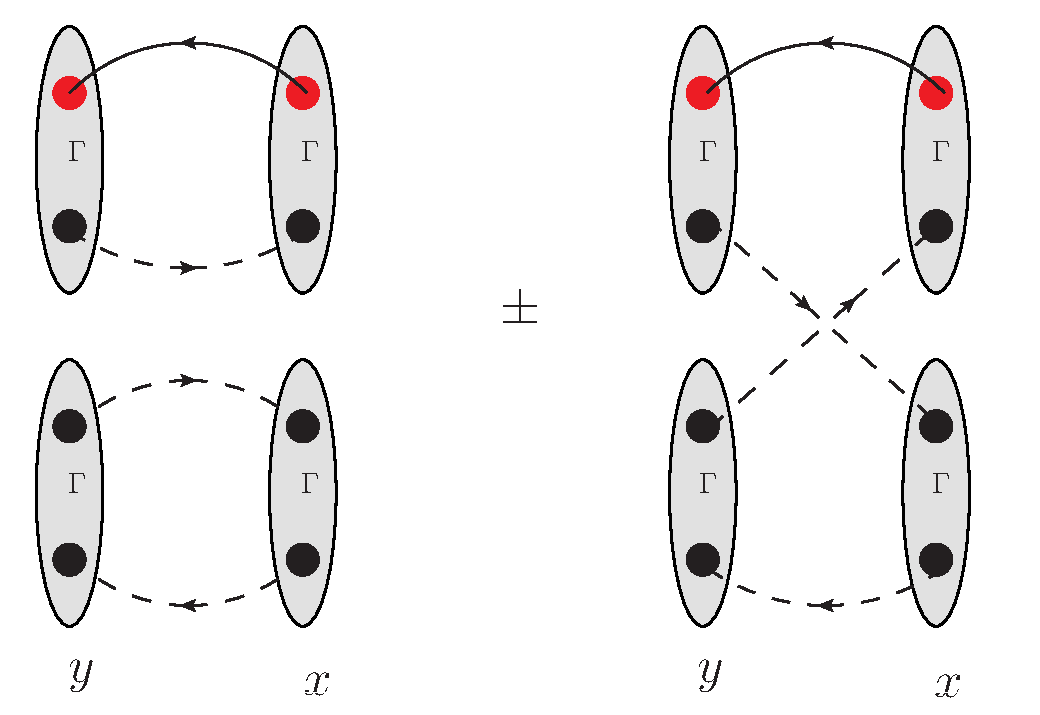
\includegraphics[width=\columnwidth]{../notes/contract1.eps}
\end{column}
\begin{column}{.6\textwidth}
\tiny
\begin{multline*}
[15]:\ \ \text{Tr}\left[\Gamma \gamma_5\mathcal{S}_{y;x}^\dag\gamma_5\Gamma\mathcal{S}_{y;x}\right]
\text{Tr}\left[\Gamma \gamma_5\mathcal{S}_{y;x}^\dag\gamma_5\Gamma\mathcal{C}_{y;x}\right]\\
-\text{Tr}\left[\Gamma \gamma_5\mathcal{S}_{y;x}^\dag\gamma_5\Gamma\mathcal{S}_{y;x}\Gamma \gamma_5\mathcal{S}_{y;x}^\dag\gamma_5\Gamma\mathcal{C}_{y;x}\right]
\end{multline*}
\begin{multline*}
[6]:\ \ \text{Tr}\left[\Gamma \gamma_5\mathcal{S}_{y;x}^\dag\gamma_5\Gamma\mathcal{S}_{y;x}\right]
\text{Tr}\left[\Gamma \gamma_5\mathcal{S}_{y;x}^\dag\gamma_5\Gamma\mathcal{C}_{y;x}\right]\\
+\text{Tr}\left[\Gamma \gamma_5\mathcal{S}_{y;x}^\dag\gamma_5\Gamma\mathcal{S}_{y;x}\Gamma \gamma_5\mathcal{S}_{y;x}^\dag\gamma_5\Gamma\mathcal{C}_{y;x}\right]
\end{multline*}
\end{column}
\end{columns}
\center
\footnotesize
$\mathcal{C}_{y;x}$ = charm quark propagator

$\mathcal{S}_{y;x}$ = light quark propagator (SU(3) point)

$\Gamma=\gamma_5\implies$ pseudoscalar

$\Gamma=\gamma_i\implies$ vector
\end{frame}

\begin{frame}{Contractions\footnote{Performed using Jan-Lukas' \texttt{form} script.} for the [$\bar{3}$]}
\center
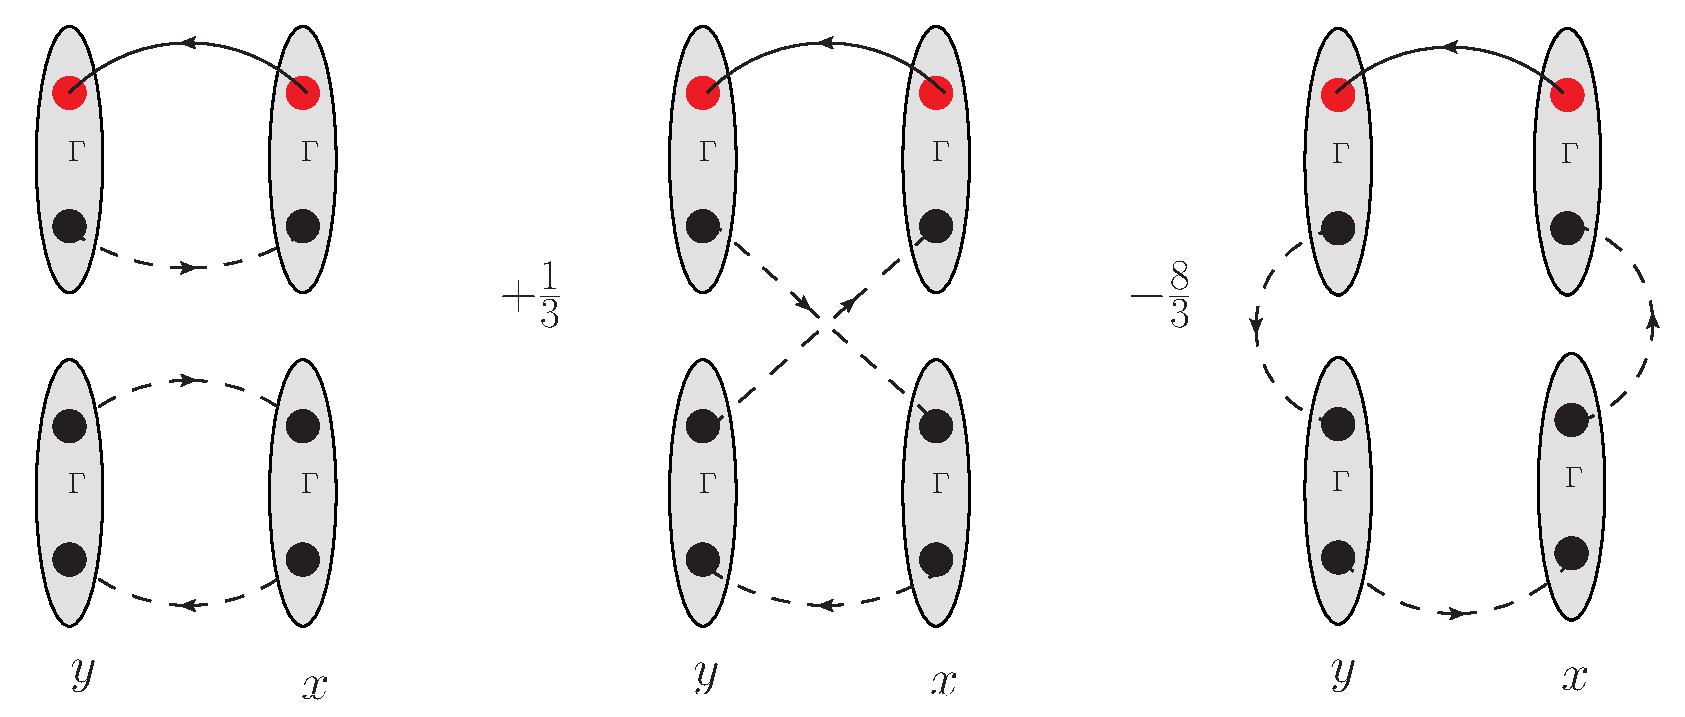
\includegraphics[width=.8\columnwidth]{../notes/contract2.eps}

\footnotesize
\begin{multline*}
[\bar{3}]:\ \ \text{Tr}\left[\Gamma \gamma_5\mathcal{S}_{y; x}^\dag\gamma_5\Gamma\mathcal{S}_{y;x}\right]
\text{Tr}\left[\Gamma \gamma_5\mathcal{S}_{y; x}^\dag\gamma_5\Gamma\mathcal{C}_{y; x}\right]\\
+\frac{1}{3}\text{Tr}\left[\Gamma \gamma_5\mathcal{S}_{y; x}^\dag\gamma_5\Gamma\gamma_5\mathcal{S}^\dag_{y; x}\gamma_5\Gamma \mathcal{S}_{y; x}\Gamma\mathcal{C}_{y; x}\right]\\
-\frac{8}{3}\text{Tr}\left[\Gamma \mathcal{S}_{x; x}\Gamma\gamma_5\mathcal{S}^\dag_{y; x}\gamma_5\Gamma {\color{red}\mathcal{S}_{y; y}}\Gamma\mathcal{C}_{y; x}\right]
\end{multline*}
\end{frame}


%\begin{frame}{Coupling with spinors}
%
%\end{frame}

\end{document}

